%% 
%% Copyright 2007, 2008, 2009 Elsevier Ltd
%% 
%% This file is part of the 'Elsarticle Bundle'.
%% ---------------------------------------------
%% 
%% It may be distributed under the conditions of the LaTeX Project Public
%% License, either version 1.2 of this license or (at your option) any
%% later version.  The latest version of this license is in
%%    http://www.latex-project.org/lppl.txt
%% and version 1.2 or later is part of all distributions of LaTeX
%% version 1999/12/01 or later.
%% 
%% The list of all files belonging to the 'Elsarticle Bundle' is
%% given in the file `manifest.txt'.
%% 
%% Template article for Elsevier's document class `elsarticle'
%% with harvard style bibliographic references
%% SP 2008/03/01

\documentclass[preprint,12pt,authoryear]{elsarticle}

%% Use the option review to obtain double line spacing
%% \documentclass[authoryear,preprint,review,12pt]{elsarticle}

%% Use the options 1p,twocolumn; 3p; 3p,twocolumn; 5p; or 5p,twocolumn
%% for a journal layout:
%% \documentclass[final,1p,times,authoryear]{elsarticle}
%% \documentclass[final,1p,times,twocolumn,authoryear]{elsarticle}
%% \documentclass[final,3p,times,authoryear]{elsarticle}
%% \documentclass[final,3p,times,twocolumn,authoryear]{elsarticle}
%% \documentclass[final,5p,times,authoryear]{elsarticle}
%% \documentclass[final,5p,times,twocolumn,authoryear]{elsarticle}

%% For including figures, graphicx.sty has been loaded in
%% elsarticle.cls. If you prefer to use the old commands
%% please give \usepackage{epsfig}

%% The amssymb package provides various useful mathematical symbols
\usepackage{amssymb}
%% The amsthm package provides extended theorem environments
%% \usepackage{amsthm}

\usepackage{graphicx} % Added package
\usepackage{siunitx} % Added package
\usepackage[version=3]{mhchem} % Added package
\usepackage{url}
\usepackage{textcomp} % Added package
% \usepackage{lineno}

%% The lineno packages adds line numbers. Start line numbering with
%% \begin{linenumbers}, end it with \end{linenumbers}. Or switch it on
%% for the whole article with 
% \linenumbers
%% \usepackage{lineno}

% \journal{Nuclear Physics B}
\journal{SoftwareX} % Changed journal

\begin{document}

\begin{frontmatter}

%% Title, authors and addresses

%% use the tnoteref command within \title for footnotes;
%% use the tnotetext command for theassociated footnote;
%% use the fnref command within \author or \address for footnotes;
%% use the fntext command for theassociated footnote;
%% use the corref command within \author for corresponding author footnotes;
%% use the cortext command for theassociated footnote;
%% use the ead command for the email address,
%% and the form \ead[url] for the home page:
%% \title{Title\tnoteref{label1}}
%% \tnotetext[label1]{}
%% \author{Name\corref{cor1}\fnref{label2}}
%% \ead{email address}
%% \ead[url]{home page}
%% \fntext[label2]{}
%% \cortext[cor1]{}
%% \address{Address\fnref{label3}}
%% \fntext[label3]{}

\title{A Scalable Database for Sensor Observations}

%% use optional labels to link authors explicitly to addresses:
%% \author[label1,label2]{}
%% \address[label1]{}
%% \address[label2]{}

\author[inst1]{Peter K. Kaiser}
\ead{p.kaiser@example.org}
\author[inst2]{John N. Doe}
\ead{j.doe@example.org}
\author[inst3]{Jutta Kaisaniemi}
\ead{j.kaisaniemi@example.org}
\address[inst1]{Environmental Informatics Research Group, University of Zurich}
\address[inst2]{Biogeochemistry Research Group, Australian National University}
\address[inst3]{College of Engineering and Computer Science, University of Eastern Finland}

\begin{abstract}
%% Text of abstract
As our main contribution, we present a scalable database capable of consuming sensor observations represented in RDF and evaluating queries for sensor observations formulated in SPARQL. We motivate the need for scalable databases for sensor observations on a case study in micrometeorology.
\end{abstract}

\begin{keyword}
%% keywords here, in the form: keyword \sep keyword
Sensor Data \sep Data Management \sep Query Performance

%% PACS codes here, in the form: \PACS code \sep code

%% MSC codes here, in the form: \MSC code \sep code
%% or \MSC[2008] code \sep code (2000 is the default)

\end{keyword}

\end{frontmatter}

%% \linenumbers

%% main text
\section{Introduction}
\label{s:introduction}
NoSQL systems have been utilized to manage sensor observations, specifically. \citet{wang14hdsw} present a Hadoop-based system designed to manage sensor observations. \citeauthor{wang14hdsw} evaluate the performance of various queries. 

Of particular interest here is CirrusRDF \citep{ladwig11cirrusrdf}. It has been widely adopted in the literature \citep{lefort12qb,phuoc11linked,mueller13restful}. The authors note that ``a complete `semantification' [...] of all data [...] seemed not feasible and promising to us, especially regarding the measurement data.'' 

As we discuss in more details in Section \ref{s:case-study}, such systems generate large volumes of data, currently stored as files.

\section{Case Study}
\label{s:case-study}
We evaluate comparative database performance with data of a typical Sensor System for the direct measurement of \ce{CO2}, \ce{CH4}, and \ce{H2O} fluxes. Large data volumes for surface-atmosphere fluxes of energy and trace gases are managed by platforms such as SOCI Portal.\footnote{The Portal is online at \url{https://www.socip.eu/} (Accessed: May 8, 2017)} The devices operate at \SI{10}{\hertz} sampling frequency and the data files include \SI{30}{\minute} of measurement. The total number of archive files is \num{1604500}. Each data file consists of a $\num{18000} \times 40$ matrix. Of this matrix, we concentrate on the three columns for measured \ce{CO2} [\si{\micro\mol\per\mol}], \ce{H2O} [\si{\milli\mol\per\mol}], and \ce{CH4} [\si{\micro\mol\per\mol}].

\begin{table}
	\centering
	\caption{A nice caption for the table.}
	\begin{tabular}{|c|r|r|r|}
		\hline
		Subset & Observations & Triples & Distinct \\
		\hline
		30 m & \num{54000} & \num{810000} & \num{648007} \\
		1 h & \num{108000} & \num{1620000} & \num{1296007} \\
		\hline 
	\end{tabular}
	\label{tbl:size-summary}
\end{table}

\begin{figure}[!ht]
  \centering
  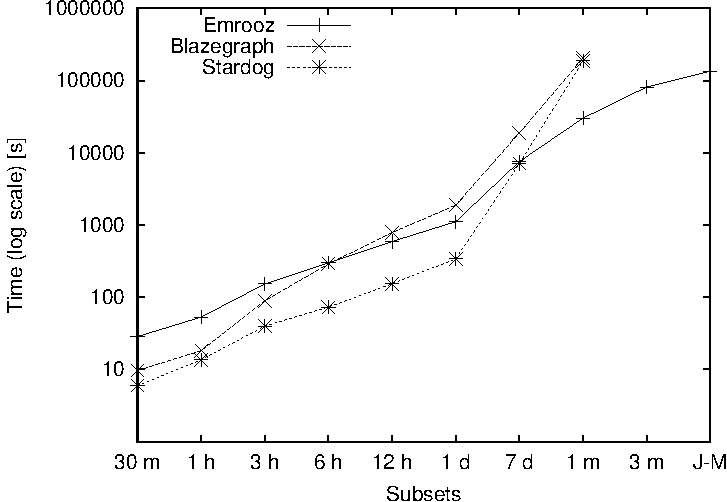
\includegraphics[scale=0.6]{load-performance-plot.pdf}
	\caption{A nice caption for the figure.}
	\label{fig:load-performance-plot}
\end{figure}

\section{Results}
\label{s:results}
Table \ref{tbl:size-summary} summarizes subset sizes in terms of number of sensor observations, corresponding triples, and distinct triples. Figure \ref{fig:load-performance-plot} summarizes the \emph{load} performance for the 10 subsets compared to Stardog and Blazegraph. Figure \ref{fig:query-performance-plot} summarizes the \emph{query} performance for the 10 subsets compared to Stardog and Blazegraph. 

The database is capable of evaluating SPARQL queries with a basic graph pattern with \texttt{FILTER} and \texttt{ORDER BY}. The query performance is determined by the following complex mathematical expression

\begin{displaymath}
\lim_{x \to a} \frac{f(x) - f(a)}{x - a}
\end{displaymath}

\begin{figure}
	\centering
	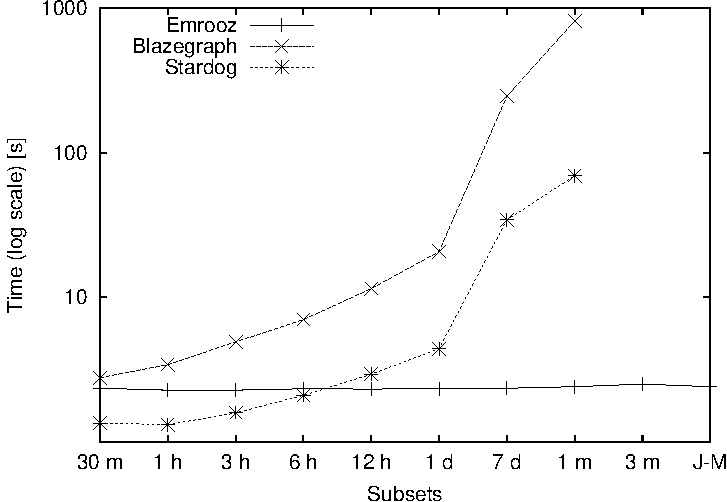
\includegraphics[scale=0.6]{query-performance-plot.pdf}
	\caption{Another nice caption for this second figure.}
	\label{fig:query-performance-plot}
\end{figure}

\section{Conclusion}
\label{s:conclusion}
We have presented a scalable database for sensor observations. That's it, folks! Thanks for reading.

\section*{Acknowledgements}
\label{s:acknowledgements}
This research is funded by the Academy of Germany project ``ROTAR: High-quality Measurement Infrastructure'' (Grant number 5489654).

%% The Appendices part is started with the command \appendix;
%% appendix sections are then done as normal sections
%% \appendix

%% \section{}
%% \label{}

%% If you have bibdatabase file and want bibtex to generate the
%% bibitems, please use
%%
\bibliographystyle{elsarticle-harv} 
% \section*{\refname} % Added, perhaps unwanted as suppressed by default?
\bibliography{bibliography}

%% else use the following coding to input the bibitems directly in the
%% TeX file.

% \begin{thebibliography}{00}

%% \bibitem[Author(year)]{label}
%% Text of bibliographic item

% \bibitem[ ()]{}

% \end{thebibliography}
\end{document}

\endinput
%%
%% End of file `elsarticle-template-harv.tex'.
